\section{EXPERIMENTS}
\label{sec:experiments}
In this section, we will evaluate our framework with different parameters and compare our method with several state-of-the-art methods on segmenting the synaptic cleft region in electron micrographs.

~\noindent\textbf{Dataset}
Synaptic images are obtained by cryo-electron tomography (CET), from which we can directly observe a native environment of synaptic structures in a high resolution (about $1500\times 1500$).
\xj{native environment or natural environment?}
%
And localizing the accurate contour of a target region in such a crowded and natural environment is significantly challenging, due to the high nose and low signal-to-noise ratio.
In this paper, our goal is to extract the synaptic cleft region, which is adjacent to a synapse and receives neurotransmitter molecules from another synapse.
Especially, only the cleft between two synapse, whose width is about $20\sim30$ nm ($40\sim70$ pixels in our electron micrographs), might be our plausible synaptic cleft.
%
For evaluating our method, we build a synaptic electron micrographs dataset, consisting $400$ synaptic images for training and $159$ images for testing.
All the image are observed in raw resolution and labeled by biomedical experts.

~\noindent\textbf{Implementation Details}
The training strategy of our DeepLab mode follows \cite{Chen2016a}.
For such a large resolution, we crop a $321\times 321$ region \cite{Chen2016} from the original image as the input to DeepLab.
In order to avoid over fitting, the training dataset is augmented by flipping and rotation, finally containing $19200$ images.

During curve evolving, $\alpha$, $\beta$, $\kappa$ and $\gamma$ are respectively set as $0.2$, $0.2$, $0.3$ and $1$, which can give a best performance in our dataset.
For synchronous growing, $\rho$ is set as $0.25$ and $\tau_1$, $\tau_2$ are $-\frac{\sqrt{2}}{2}$, $\frac{\sqrt{2}}{2}$ to constraint the direction of a new piece of contour to deviating $[-\frac{\pi}{4},\frac{\pi}{4}]$ from last growing direction.
And when $d^{t}$ is beyond the range of $[40,80]$, the growing is terminated.

We use two metrics \cite{Cheng2017} to evaluate our method on segmentation task:
a) pixel accuracy, which evaluates the percentage of positive true pixels over the whole pixels;
b) pixel intersection-overunion (IOU) averaged across different classes.

\begin{figure}[t]
\begin{center}
        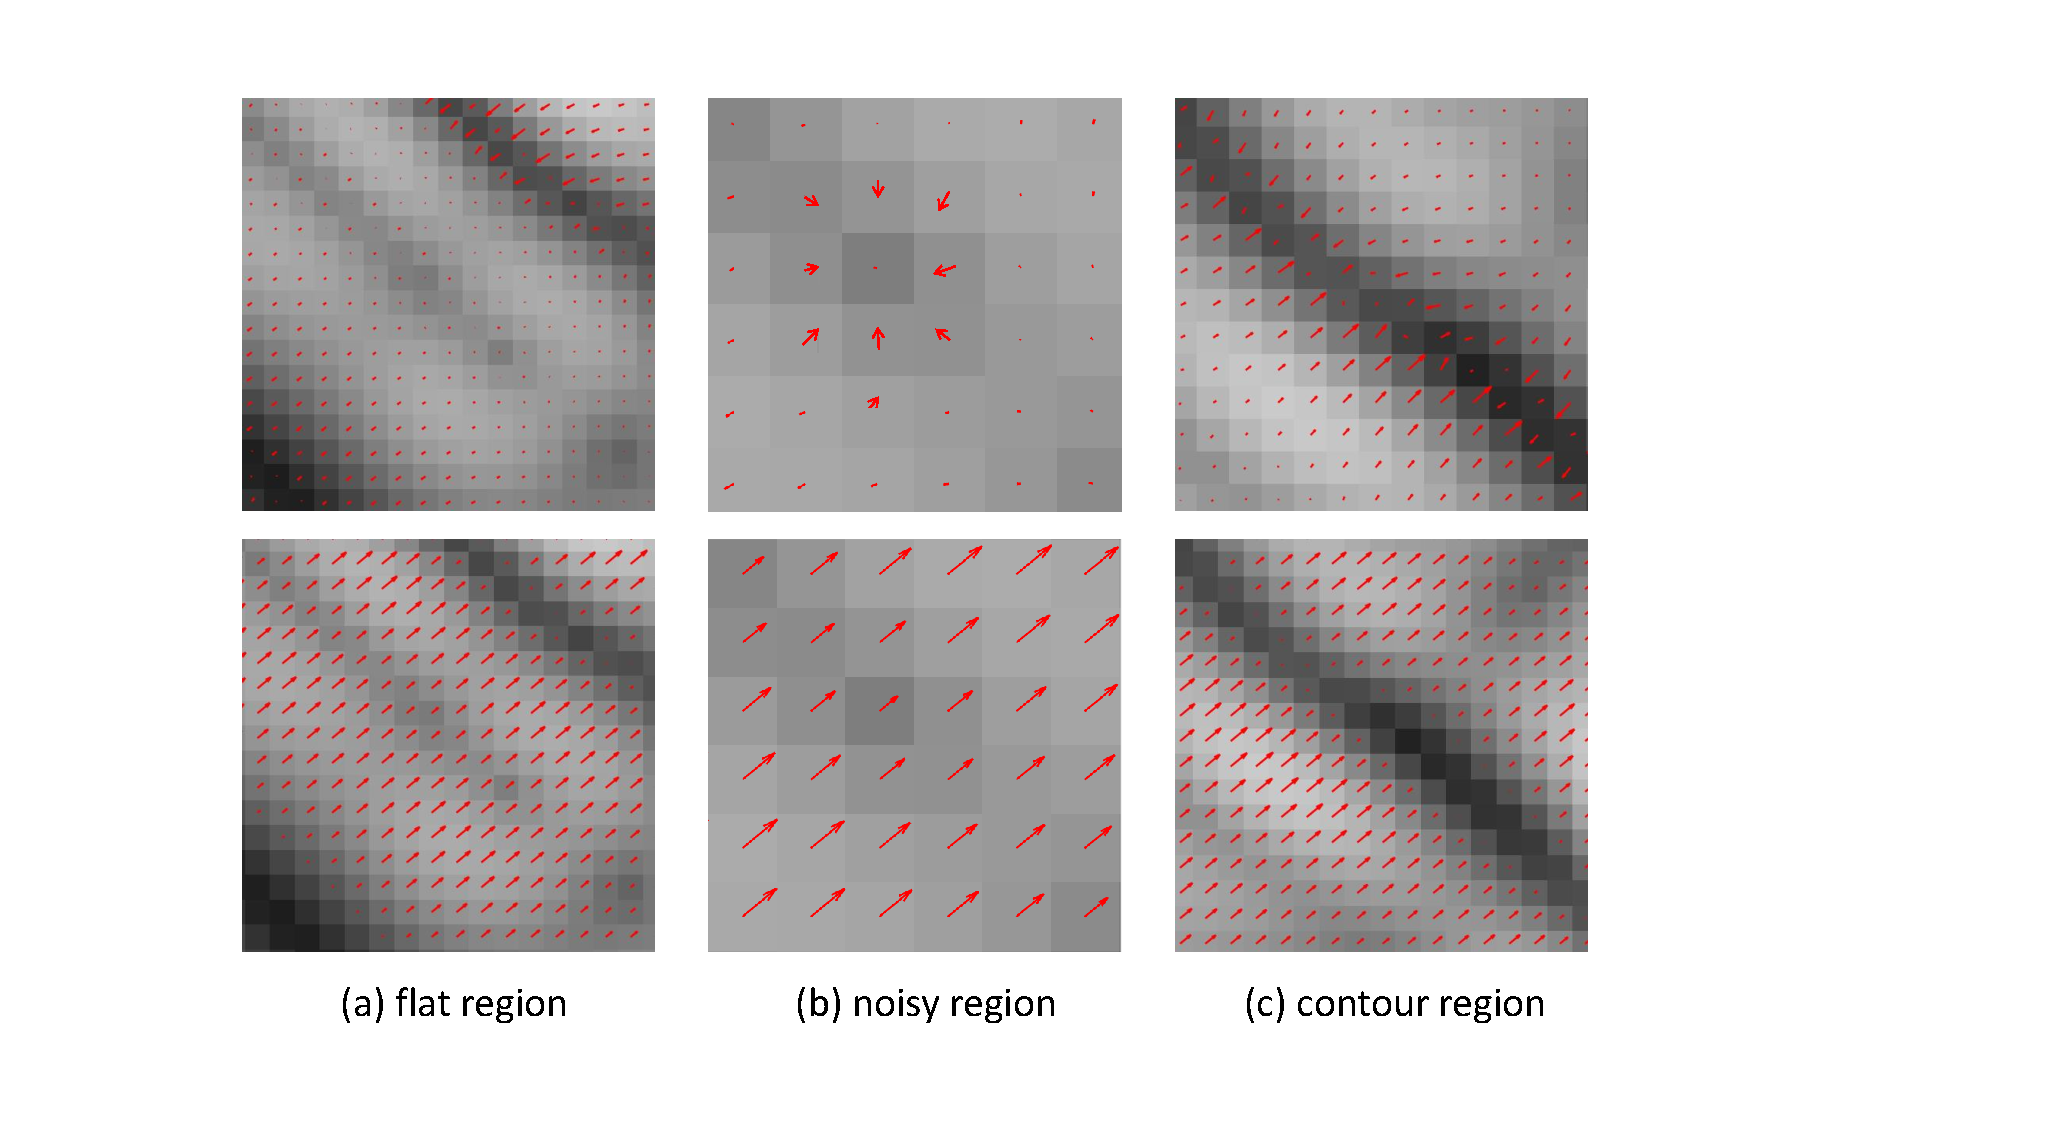
\includegraphics[width=3.4in]{figs/FigGVF.pdf}
   \end{center}
%
\caption{Several cases of tension field obtained by GVF (top row) and our normal force (bottom row). The red arrow indicates the force vector of external tension.}
\label{fig:gvf}
\end{figure}
~ \noindent\textbf{Superiority of Eq.~\ref{Eq:update}.}
In this part, we visualize the deficiencies of traditional updating Eq.~\ref{Eq:GVF} in GVF and represent the superiority of our strategy of Eq.~\ref{Eq:update}.
Firstly, in some flat regions with small gradients $\mathbf{f}$, the external tension is too weak to drive $\mathbf{v}(s)$ to move against to internal tension.
Therefore, it requires the initial curve to be away from the flat regions (Fig.~\ref{fig:gvf} (a)).
Secondly, the external tension in some noisy regions will be gyrate, which easily trap some $\mathbf{v}(s)$ (Fig.~\ref{fig:gvf} (b)).
Although sometimes the internal tension may pull the trapped point out, the gyrate $\mathbf{f}$ will trap it again.
And using Eq.~\ref{Eq:update} , once $\mathbf{v}(s)$ is pulled away from the noisy region, our external tension with fixed normal direction will soon push it away.
Thirdly, as the gradients $\mathbf{f}$ near to contours are usually large (Fig.~\ref{fig:gvf} (c)), $\mathbf{v}(s)$ easily cross the optimal positions by over-huge tension, while our external tension are controlled by $E_{ext}$, which will soon vanish in contour region and make the updating more robust.

~\noindent\textbf{Results}
We evaluate the state of the art segmentation methods, including FCN \cite{Long2015}, U-net \cite{Ronneberger2015}, DeepLab (vgg16, ResNet-101) \cite{Chen2016a} and PSPNet \cite{Zhao2016}, with our proposed model on segmenting synaptic cleft region.

Table~\ref{tab:report1} reports the pixel accuracy and mean IOU of different methods, while Fig.~ represents some visual instances of these methods.
From Table~\ref{tab:report1}, it can be found that our model gives the best performance among existing methods and our localized contours are much more precise and complete than single FCN based methods in Fig..
Especially, Unet performs better than FCN and DeepLab(vgg16), due to richer features extracted by U-shaped architecture.
The effects of pyramid pooling module used in PSPNet are not obvious compared to DeepLab(ResNet-101) in our task.
And the results of DeepLab(ResNet-101) and PSPNet are better than other FCNs, which demonstrate the effectiveness of deeper ResNet.
From Fig. , FCNs can localize the correct positions of synaptic cleft in most cases, but their contours are not precise enough for further analysis.

\begin{table}[t]
\begin{center}
\caption{Table caption} \label{tab:report1}
\begin{tabular}{|c|c|c|}
  \hline
  % after \\: \hline or \cline{col1-col2} \cline{col3-col4} ...
   & Pixel Accu. & mean IOU
  \\
  \hline
  FCN & 0.9923 & 0.5258 \\
  Unet &  0.9939 & 0.6359 \\
  DeepLab(Vgg16) & 0.9838 & 0.5867 \\
  DeepLab(ResNet-101) & 0.9951 & 0.7164 \\
  PSPNet & Cell 5 & Cell 6 \\
  Contour Growing & $\mathbf{0.9974}$ & $\mathbf{0.7848}$ \\
  \hline
\end{tabular}
\end{center}
\end{table}

Furthermore in order to prove the robustness of our model to initial segmentation, we explore the effects of different pre-segmentation model to our contour growing results.
It should be noted that DeepLab in Table~\ref{tab:report2} indicates the ResNet101 version of DeepLab, which is our default pre-segmentation network.
From the results in Table~\ref{tab:report2}, it demonstrates that our contour growing algorithm can obviously improve the results of different pre-segmentation model.
And observed from Fig.~\ref{}, as long as the correct location of synaptic cleft region is provided (Unet, DeepLab and PSPNet), our model can well localize the whole contours of target region.

\begin{table}[t]
\begin{center}
\caption{Table caption} \label{tab:report2}
\begin{tabular}{|c|c|c|}
  \hline
  % after \\: \hline or \cline{col1-col2} \cline{col3-col4} ...
   & Pixel Accu. & mean IOU
  \\
  \hline
  Contour Growing$+$FCN & 0.9956 & 0.6339 \\
  Contour Growing$+$Unet & 0.9962 & 0.7720 \\
  Contour Growing$+$DeepLab & 0.9974 & 0.7848 \\
  Contour Growing$+$PSPNet & Cell 5 & Cell 6 \\
  \hline
\end{tabular}
\end{center}
\end{table}
